% scenarios2.tex
% --
% James Jackson <eeu203@bangor.ac.uk>



% We want this to be an article
\documentclass[pdftex,a4paper,10pt,titlepage]{article}

% Outline the packages to be used (natbib, fancyhdr, url, geometry, hyperref)
\usepackage[utf8]{inputenc}
\usepackage[round,authoryear,sort]{natbib}
\usepackage{fancyhdr}
\usepackage[margin=0.5in]{geometry}
\usepackage[hidelinks]{hyperref}
\usepackage[anythingbreaks]{breakurl}
\usepackage{graphicx}
\usepackage{hyperref}
\usepackage{amsmath}

\graphicspath{ {.} }



\setcounter{secnumdepth}{4}


% Begin the document
\begin{document}








% Set up page style for fancy headers, along with the header information (and page width!)
\newgeometry{margin=1in}
\pagestyle{fancy}
\fancyhf{}
\lhead{James Jackson - eeu203}
\rhead{ICP-2036}
\cfoot{\thepage}




\section{Description}
\subsection{Loading Data}
The program created allows the user to select any “.raw” file and visualise the data. Due to limitations in the .raw formats meta data it is easy to decipher the dimensions of the data held within and as such it is necessary for the user to supply this information prior to loading the file. 
Views
Once loaded the user will be presented with 6 visual representations of the data 
\begin{itemize}
\item 3 orthogonal planes scrolling along the x, y and z axes respectively.
\item 3 non-orthogonal planes slicing at angles down the x, y and z axes.
\end{itemize}
Each view contains two control elements, a slider to iterate through the given axis or angle and a combo box to allow a user to control the view’s color profile.

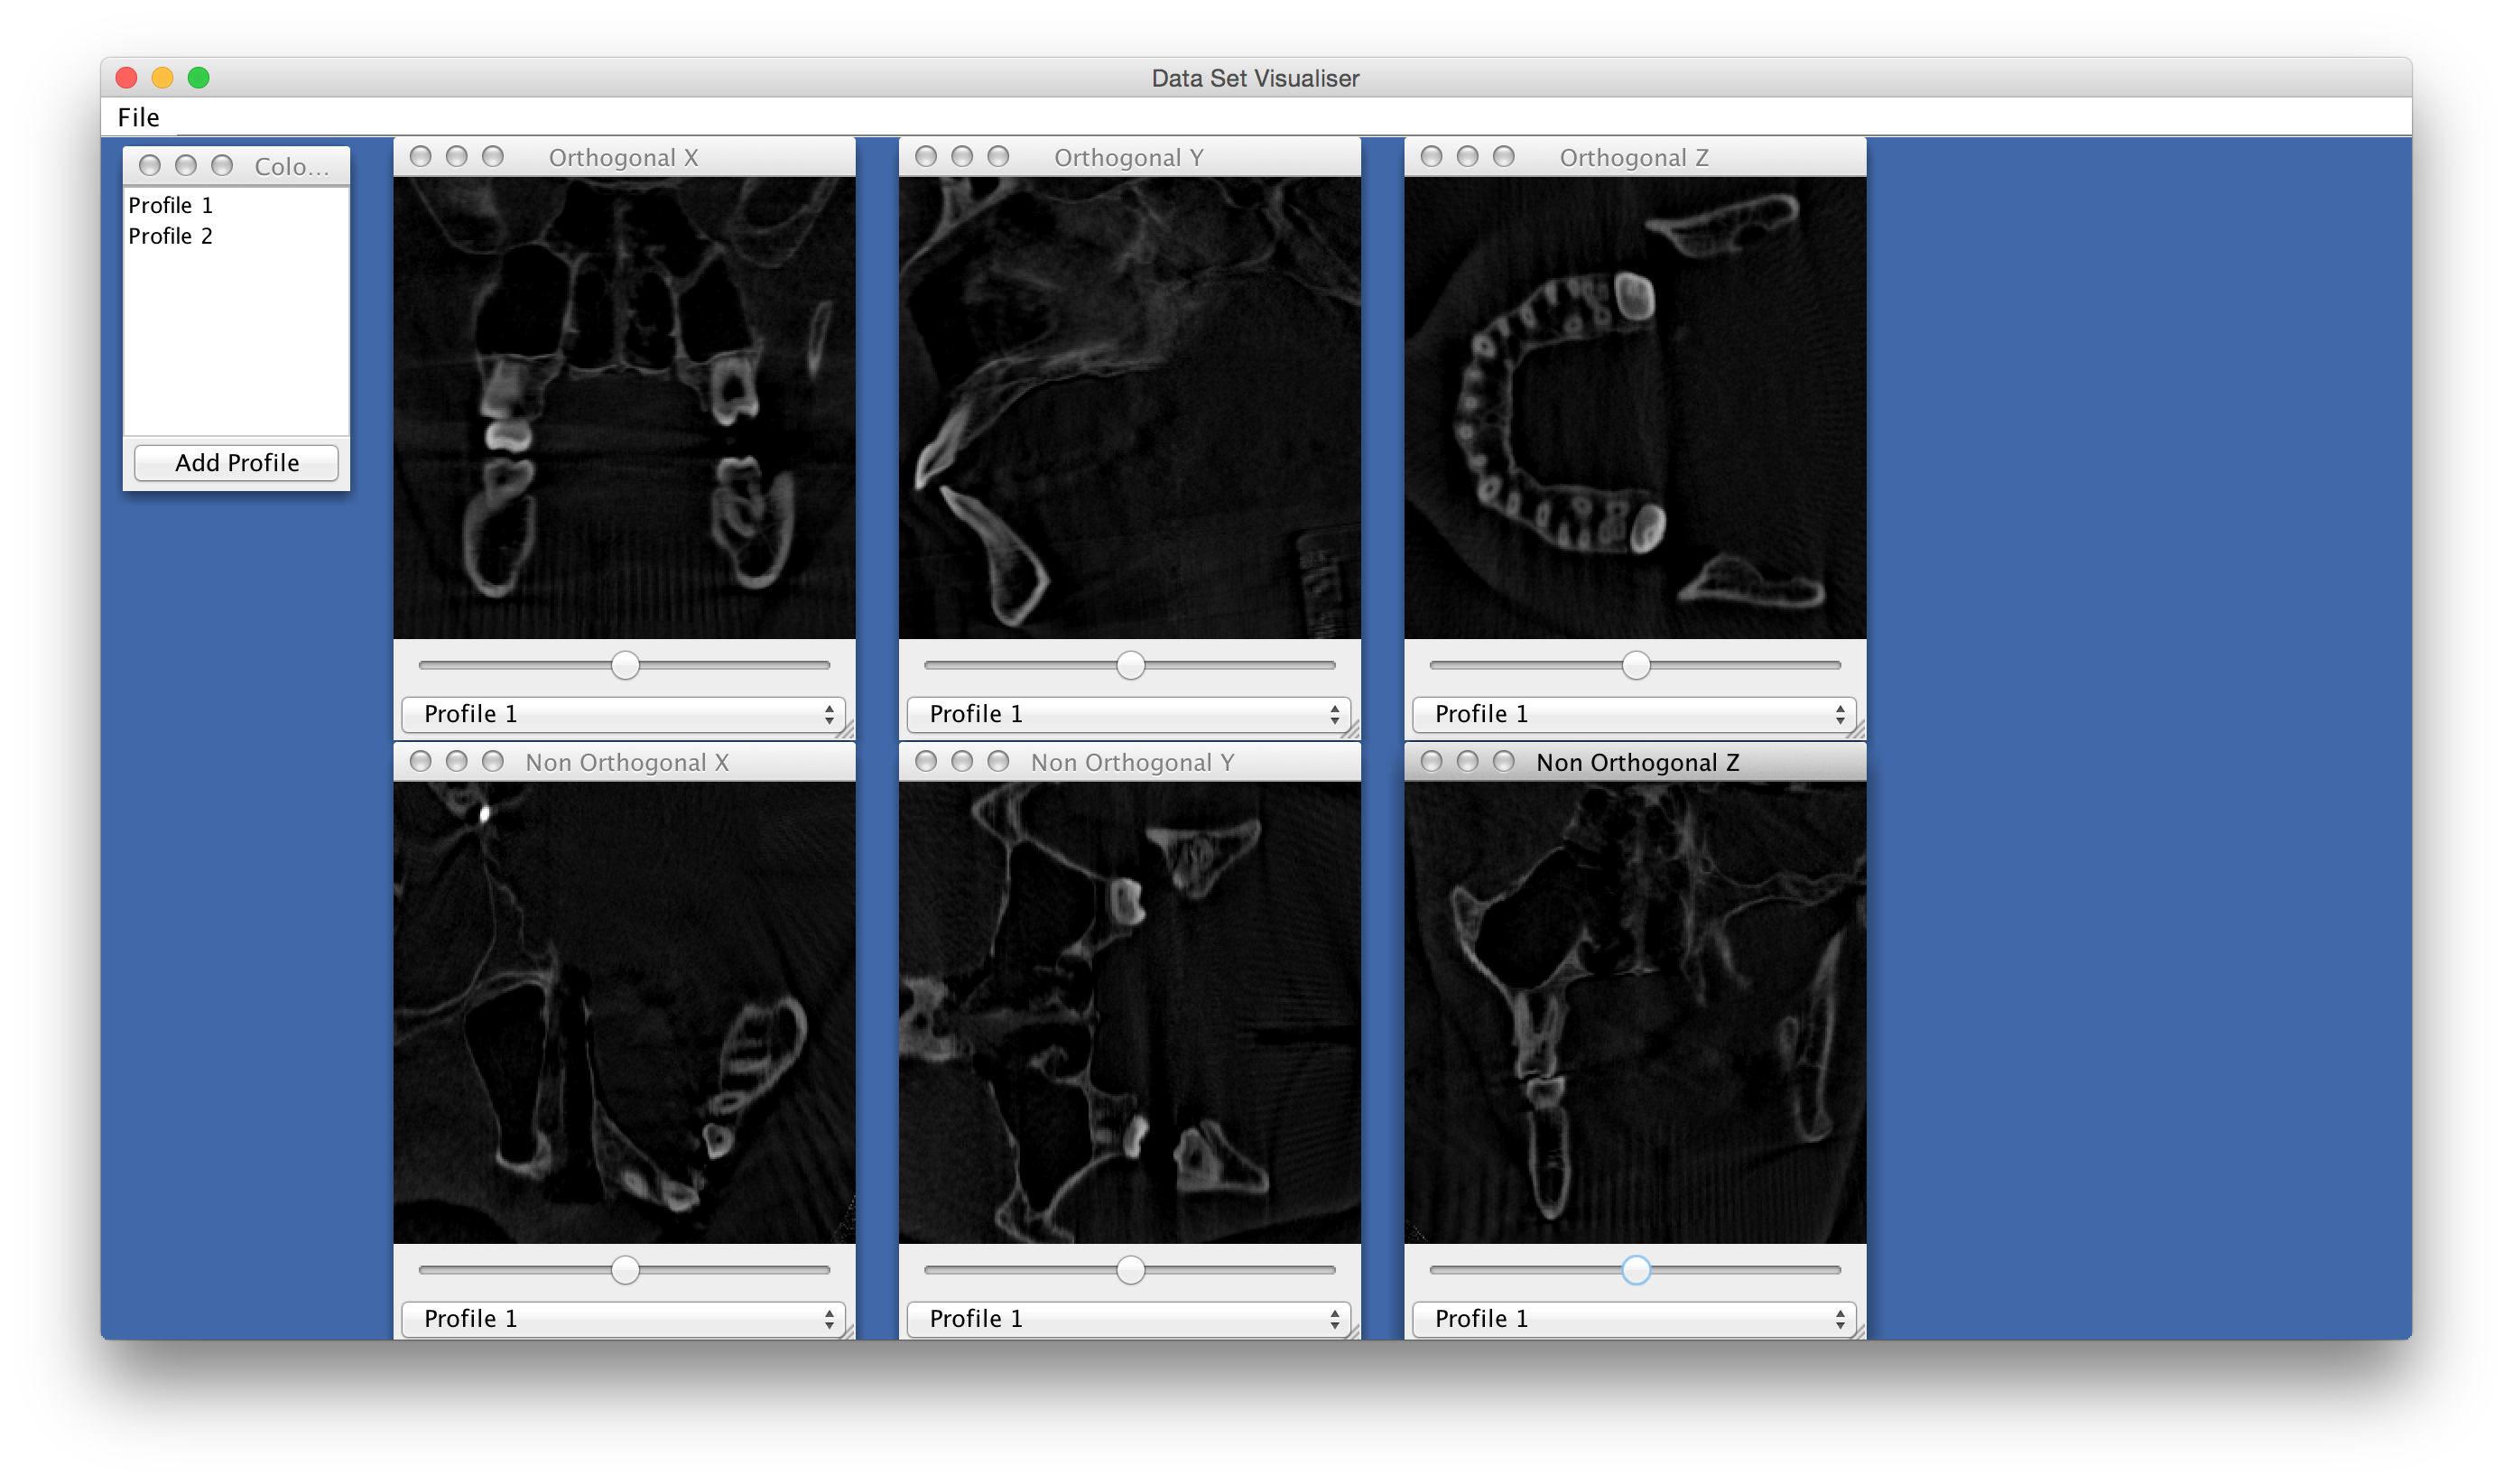
\includegraphics[width=\textwidth]{screen1}

\subsection{Color Profiles}
A user is able to create color profiles to be used across the views. These profiles work by the user selecting colors for a selected key data values, the view will the interpolate between these color steps to produce the desired color. e.g. consider the following color profile (integer RGB values)
\begin{equation*}
0 - 0,0,0 (Black)
\end{equation*}
\begin{equation*}
120 - 255, 0 , 0 (Red)
\end{equation*}
\begin{equation*}
255 - 255, 255, 255 (White)
\end{equation*}
There are 128 steps between the first two key steps so each step will calculate its own color based on the following:
let m = current data value, c = n’s color, n = first data value in current range, o = the last value in the current range,
\begin{equation*}
c = n.color + (o.color - n.color / o - n) * m - n
\end{equation*}
So if m = 80: c = (0, 0, 0) + (2.125, 0, 0) * 80 = 170, 0, 0
At any point a user can create and use new color profiles to use on the various views.
\pagebreak
\section{Critical Analysis}
\subsection{Strengths}
There are various strengths in this application:
\subsubsection{Simple To Load}
Removing the step where a user selects a plane takes away ambiguity that may pop up in a user’s misunderstanding of the various axes and planes.
\subsubsection{Color Profiles}
Initially color steps were saved independently to each view meaning a user couldn’t select that profile on a different view, color profiles are view independent.
\section{Weaknesses}
There are a few issues with the application that could be rectified or ironed out in future iterations. 
\subsection{Functionality}
There are various desired facets that are not present in the final application which were omited due to time constraints\\
\textbf{Loading}
When a user loads the data files there is no obvious depiction of the file loading, this could lead to the user not thinking that anything is happening. \\
\textbf{Single Larger View}
An early plan for the application was to allow the user to select an active view and see a much larger rendition of it. \\
\textbf{Mousewheel Control}
Allowing the user to control the current slider through the use of the mouse wheel would have been beneficial to allow the user a more intuitive experience.\\
\textbf{Zoom}
Originally planned as part of the single large view, this would have allowed the user to zoom into a given view.\\
\textbf{Current Plane Depiction}
Showing a visual representation of the current plane is a much more simple and easy to understand that text representations.
\subsection{Coding}
\textbf{Loops}
Various points in the code are utilising nested for loops, these could be replaced with single loops to speed up execution.\\
\textbf{Floating Points}
In various points of the application floating point arithmetic is used. Converting the floating point calculations to integer calculations would also allow for faster execution.












% End the document
\end{document}